\documentclass[french]{article}
\usepackage[utf8x]{inputenc}
\usepackage[T1]{fontenc}
\usepackage{babel}
\usepackage{lmodern}
\usepackage[top=2cm,bottom=2cm,left=3cm,right=3cm]{geometry}
\usepackage{microtype}
\usepackage{mathtools, amssymb, amsthm}
\usepackage{mdframed}
\usepackage{hyperref}
\usepackage{graphicx}
\usepackage{xcolor}
\usepackage{mathrsfs}
\usepackage{wrapfig}
\usepackage{stmaryrd}
\usepackage{dsfont}
\usepackage{framed}
\usepackage[Glenn]{fncychap}

\newtheorem{prototheorem}{Théorème}[section]
\newenvironment{thm}
   {\colorlet{shadecolor}{orange!10}\begin{shaded}\begin{prototheorem}}
   {\end{prototheorem}\end{shaded}}

\newtheorem*{protocorollary}{Corollaire}
\newenvironment{corollary}
    {\colorlet{shadecolor}{violet!10}\begin{shaded}\begin{protocorollary}}
    {\end{protocorollary}\end{shaded}}

\newtheorem*{protolemma}{Lemme}
\newenvironment{lemma}
    {\colorlet{shadecolor}{pink!15}\begin{shaded}\begin{protolemma}}
    {\end{protolemma}\end{shaded}}

\theoremstyle{definition}
\newtheorem{protodefinition}{Définition}[section]
\newenvironment{definition}
    {\colorlet{shadecolor}{green!5}\begin{shaded}\begin{protodefinition}}
    {\end{protodefinition}\end{shaded}}

\newtheorem{protoproposition}{Proposition}[section]
\newenvironment{prop}
    {\colorlet{shadecolor}{blue!5}\begin{shaded}\begin{protoproposition}}
    {\end{protoproposition}\end{shaded}}

\theoremstyle{remark}
\newtheorem*{remark}{Remarque}
\newtheorem{exo}{Exercice}
\newtheorem*{protoexemple}{Exemple}
\newenvironment{exemple}
    {\colorlet{shadecolor}{gray!10}\begin{shaded}\begin{protoexemple}}
    {\end{protoexemple}\end{shaded}}


\newcommand{\lesss}{\rotatebox[origin=c]{90}{$\land$}}
\newcommand{\less}{\ \lesss\ }

\newcommand{\biggg}{\rotatebox[origin=c]{90}{$\lor$}}
\newcommand{\bg}{\ \biggg\ }

\title{\bsc{Tutoriel Atom + \LaTeX}}
\date{2023}

\begin{document}

\maketitle

\tableofcontents

\section{Introduction}

Cette présentation a pour but d'expliquer comment on peut taper en LaTeX vite grâce au logiciel Atom (Pulsar).

J'ai commencé à taper mes cours magistraux en LaTeX lorsque j'ai commencé mon année de Licence 3. Vous pouvez consulter mes notes de cours de M1 \href{https://github.com/volkhovcossack/M1-AAPM}{en suivant ce lien}. L'intégralité du contenu a été écrit pendant les cours, sauf  des remarques personnelles qui ont été ajoutées après relecture.

Cet article ne s'adresse pas uniquement aux étudiants qui veulent taper leurs cours en LaTeX, mais aussi à tous ceux qui utilisent beaucoup ce logiciel. Je vais axer ma présentation sur la prise de notes en LaTeX pour montrer quelle vitesse on peut développer en utilisant cette méthode.

Cet article rend hommage à Gilles \bsc{Castel}, l'étudiant qui a popularisé la prise de notes en LaTeX et décédé en 2022. Vous pouvez consulter son tutoriel \href{https://castel.dev/post/lecture-notes-1/}{sur son blog}.

\subsection{Objectifs}

Il faut garder un seul et unique objectif en tête : taper aussi vite que le professeur écrit au tableau. Clairement, cela ne sert à rien de venir avec un ordinateur en classe si c'est pour rater les trois quarts du contenu à cause des commandes qu'on aura cherché et des fautes de syntaxe qu'on aura débugué.

\subsection{Prérequis}

La prise de notes en LaTeX ne se fait pas à l'improviste, mais on ne demande pas des connaissances non accessibles au commun des mortels. Il faut savoir écrire et structurer un document mathématique et savoir débuguer les erreurs les plus courantes (qui sont clairement des erreurs de syntaxe).

\section{Atom}

Atom est un éditeur de texte personnalisable et gratuit qui fonctionne sous Windows, Linux et Mac. Malheureusement, en 2022 Github a arrêté le projet Atom, mais la communauté continue à maintenir l'éditeur sous le nom de Pulsar (qui est très similaire à Atom).

\subsection{Les packages LaTeX}

Pour utiliser LaTeX dans Atom (Pulsar), on a besoin d'installer les packages suivants :

\begin{enumerate}
  \item language-latex : pour la syntaxe LaTeX ;
  \item latex : pour compiler.
\end{enumerate}

On peut aussi installer des packages optionnels :

\begin{enumerate}
  \item autocomplete-latex : pour avoir certains snippets (on en reparlera dans la section \ref{snippets}) ;
  \item pdf-view : pour afficher les documents .pdf directement dans Atom ;
  \item atom-latex : pour une compilation plus simple que l'on peut faire via la fenêtre ``Packages > Atom-LaTeX > Build LaTeX''.
\end{enumerate}

Ce sont les packages principaux que j'utilise, il existe aussi d'autres packages qui fonctionnent avec LaTeX et que l'on peut consulter \href{https://gist.github.com/Aerijo/5b9522530715e5be6e89fc012e9a72a8}{ici}.

Voici à quoi ressemble l'éditeur Atom une fois tous les packages installés :

\begin{figure}[h!]
  \centering
  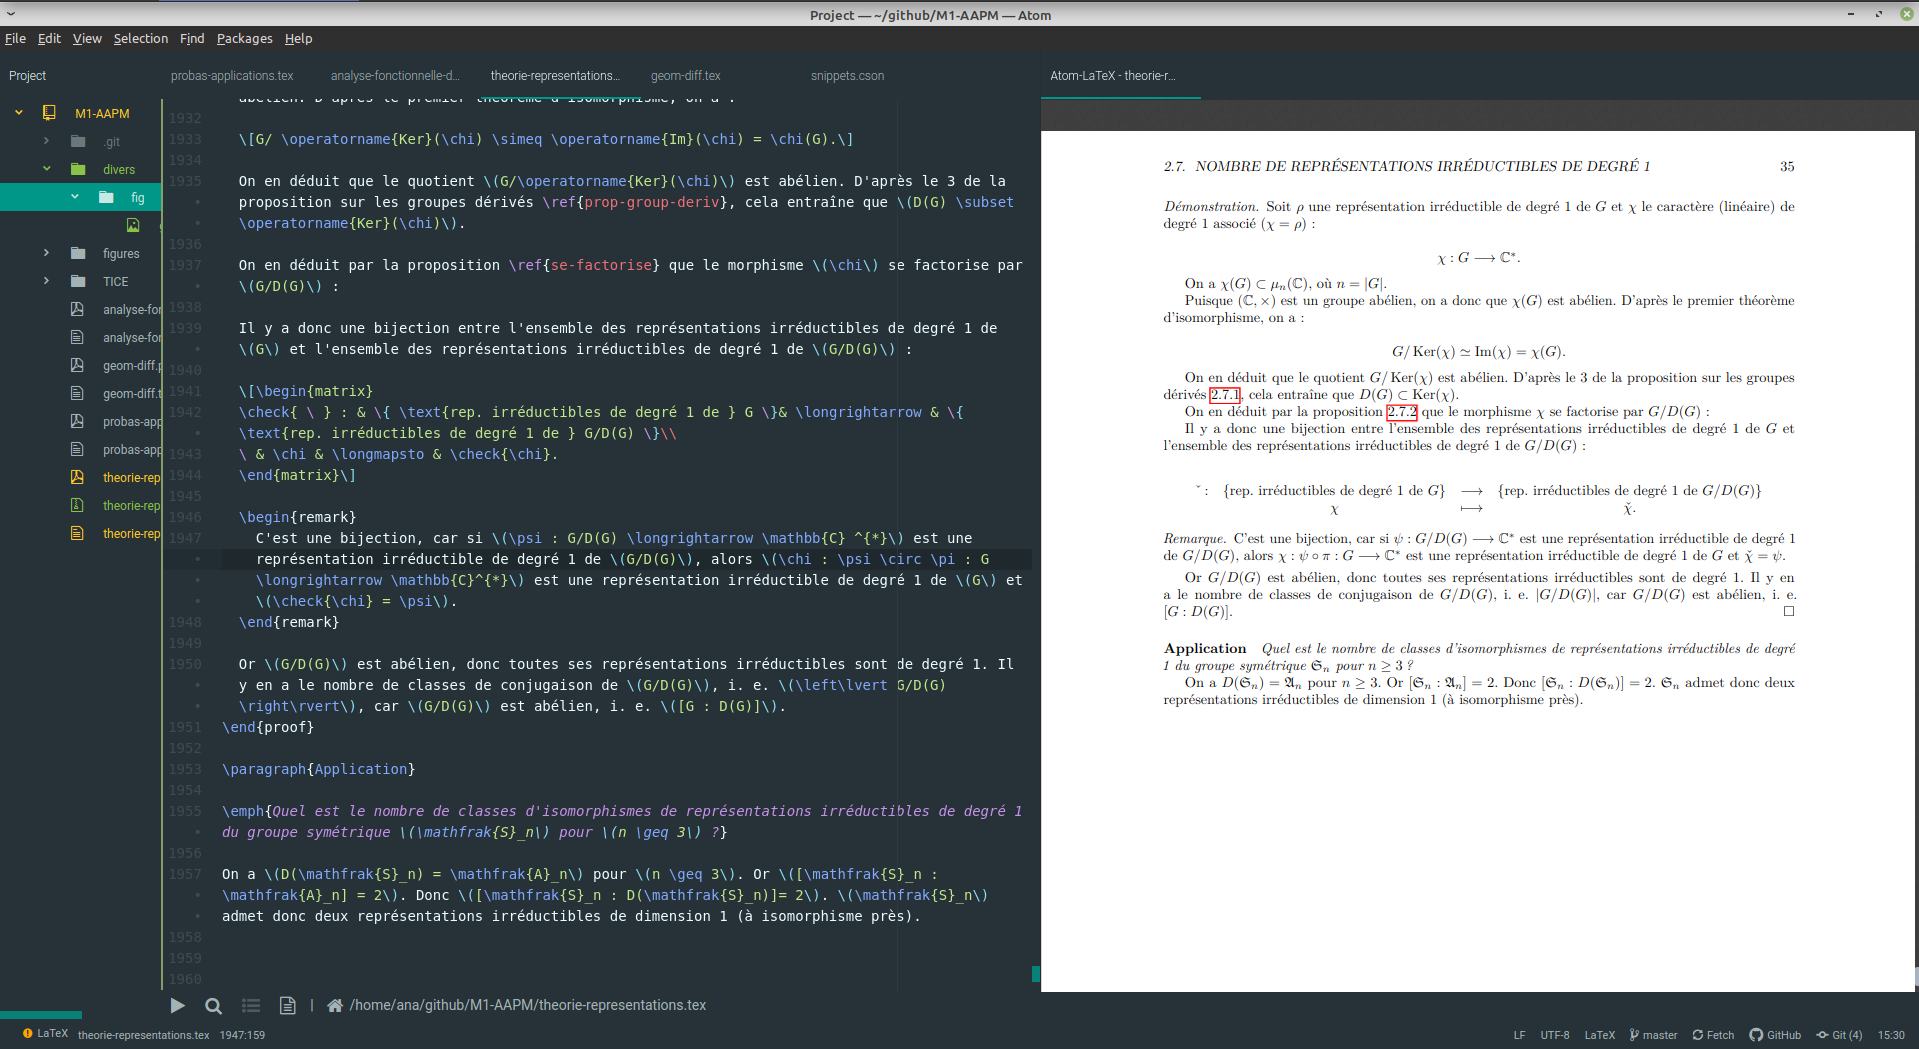
\includegraphics[scale=0.2]{fig/general.png}
  \caption{Vue d'ensemble}
  \label{}
\end{figure}

On peut installer les packages de deux manières :

\begin{enumerate}
  \item En allant dans ``Packages > Setting View > Install'' et en cherchant le package souhaité ;
  \item En tapant dans le terminal (pour Pulsar) :

  \begin{verbatim}
    ppm install nom_du_package
  \end{verbatim}
\end{enumerate}

\section{Snippets} \label{snippets}

Un \emph{snippet} est un morceau de code que l'on peut réutiliser et qui peut être activer en faisant une autre combinaison de touches plus simple.

Par exemple, si on tape ``bla'' et on presse la touche ``Entrée'', on aura ``blablablablabla''.

Un snippet peut être utilisé dans un autre. Si on combine le snippet ``txt'' qui donne ``truc  machin'' (avec un texte à écrire au milieu) avec le snippet ``bla'', on aura ``truc blablablablabla machin''.

\subsection{Comment faire un snippet dans Atom}

Pour créer un snippet dans Atom, il faut aller dans ``Edit > Snippets''. Le fichier nommé ``snippets.cson'' s'ouvrira. Il est vide au début et c'est à l'utilisateur de le remplir.

Pour commencer à taper ses propres snippets, on doit écrire au début du fichier

\begin{verbatim}
  '.text.tex.latex':
\end{verbatim}

pour bien préciser à la machine que les snippets ne concerneront que les fichiers .tex.

Les snippets dans Atom ont la structure suivante :

\begin{verbatim}
  'Nom du snippet':
    'prefix':'combinaison de touches'
    'body':"""
    Morceau de code
    """
\end{verbatim}

{\fontencoding{U}\fontfamily{futs}\selectfont\char 66\relax} Il faudra enregistrer préalablement les fichiers sous format .tex pour pouvoir utiliser les snippets.

De plus, pour utiliser les snippets à la suite du texte qu'on écrit, il faudra séparer le dernier mot et le snippet avec un espace.


\subsection{Les snippets simples}

On peut créer des snippets pour les symboles mathématiques les plus courants  comme \(\times, \circ, \geq, \leq \) ainsi que pour des ensembles \(\mathbb{R}, \mathbb{C}, \mathbb{N}, \dots\) On voudrait que l'écriture de ses symboles soit la plus simple possible, par exemple ``R'' pour \begin{verbatim}
  \mathbb{R}
\end{verbatim}

Voici comment on écrit ce snippet :

\begin{figure}[h!]
  \centering
  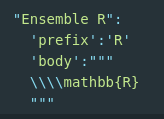
\includegraphics[scale=0.5]{fig/snipr.png}
  \caption{Snippet \(\mathbb{R}\)}
  \label{}
\end{figure}

Ainsi, lorsqu'on tapera ``R''+Entrée, on obtiendra \(\mathbb{R}\). Notez bien que pour faire apparaître un antislash, il faudra en taper 4 dans le fichier ``snippets.cson''.

\subsection{Les snippets plus complexes}

Si l'on veut créer des snippets pour les environnements comme les définitions, les théorèmes, etc, le snippet nous dirigera automatiquement à la fin de

\begin{verbatim}
\end{environnement}
\end{verbatim}

Pour plus de confort, on aimerait bien que l'on soit dirigé à l'intérieur de l'environnement, à savoir entre

\begin{verbatim}
\begin{environnement}
\end{verbatim}

et

\begin{verbatim}
\end{environnement}
\end{verbatim}

Pour cela, on devrait écrire dans le snippet

\begin{verbatim}
  ${1:}
\end{verbatim}

Par exemple, pour le snippet ``Théorème'' défini ci-dessus, on a :

\begin{verbatim}
  'Théorème':
    'prefix':'thm'
    'body':"""
    \\\\begin{thm}
      ${1:}
    \\\\end{thm}
    """
\end{verbatim}

On peut aussi taper, après ``:'', un texte pour se rappeler ce que l'on devrait écrire. Le snippet ``Théorème'' précédent deviendra alors :

\begin{verbatim}
  'Théorème':
    'prefix':'thm'
    'body':"""
    \\\\begin{thm}
      ${1:contenu}
    \\\\end{thm}
    """
\end{verbatim}

On peut aussi définir plusieurs ``morceaux'' importants du snippet. Par exemple, pour le snippet ``Définition'', il y a une partie qui correspond au nom et une autre au contenu. Pour cela, on a besoin de taper :

\begin{verbatim}
  'Définition':
    'prefix':'def'
    'body':"""
    \\\\begin{definition}[${1:}]
      ${2:}
    \\\\end{definition}
    """
\end{verbatim}

On peut ainsi définir plusieurs ``morceaux importants'' dans le snippet. Par exemple, pour le snippet ``définir fonction'' qui permet d'écrire une fonction avec l'ensemble de départ et l'ensemble d'arrivée, j'ai écrit le code suivant :

\begin{verbatim}
  'définir fonction':
    'prefix':'fct'
    'body':"""
    \\\\begin{matrix}
    ${1:nom} : & ${2:départ} & \\\\longrightarrow & ${3:arrivée} \\\\\\\\
    \\\\ & ${4:variable} & \\\\longmapsto & ${5:expression}
    \\\\end{matrix}"""
\end{verbatim}

\subsection{Les snippets les plus courants}

\subsubsection{Puissance et indice}

Pour mettre un indice, je tape simplement ``yy'' et j'obtiens

\begin{verbatim}
  _{}
\end{verbatim}

J'ai écrit ce snippet de la manière suivante dans ``snippets.cson'' :

\begin{verbatim}
  'Indice':
    'prefix':'yy'
    'body':"""
    _{${1:}}
    """
\end{verbatim}

Pour les puissances, j'utilise la combinaison ``pp''. J'ai défini ce snippet comme suit :

\begin{verbatim}
  'Puissance':
    'prefix':'pp'
    'body':"""
    ^{${1:}}
    """
\end{verbatim}

Pour les puissances les plus courantes comme le carré, le cube et l'inverse, voici les snippets correspondants :

\begin{enumerate}
  \item Carré :

  \begin{verbatim}
    'Carré':
      'prefix':'2'
      'body':"""^2"""
  \end{verbatim}

  \item Cube :

  \begin{verbatim}
    'Cube':
      'prefix':'3'
      'body':"""^3"""
  \end{verbatim}

  \item Inverse :

  \begin{verbatim}
    'Inverse':
      'prefix':'inv'
      'body':"""
      ^{-1}"""
  \end{verbatim}
\end{enumerate}

\subsection{Fractions, sommes, limites}

Pour écrire les fractions plus vite, j'ai défini un snippet qui s'active lorsque je tape ``frac''. Voici le code correspondant :

\begin{verbatim}
  "Fraction":
    'prefix':'frac'
    'body':"""
    \\\\frac{${1:}}{${2:}}
    """
\end{verbatim}

Pour les sommes, voici le code :

\begin{verbatim}
  "Sum":
    'prefix':'sum'
    'body':"""
    \\\\sum_{${1:}}^{${2:}}
    """
\end{verbatim}

J'ai une commande spéciale pour les séries numériques :

\begin{verbatim}
  "Serie":
    'prefix':'serie'
    'body':"""
    \\\\sum_{n=1}^{\\\\infty} ${1:}
    """
\end{verbatim}

Pour écrire les limites, je tape juste ``lim'' et j'obtiens

\begin{verbatim}
  \lim_{ \to}
\end{verbatim}

Pour cela, il faudra écrire :

\begin{verbatim}
  'Limite':
    'prefix':'lim'
    'body':"""
    \\\\lim_{${1:} \\\\to} ${2:}
    """
\end{verbatim}

J'ai une commande spéciale pour les limites des suites qui tendent vers l'infini en \(n\) :

\begin{verbatim}
  'Limite_n':
    'prefix':'limn'
    'body':"""
    \\\\lim_{n \\\\to \\\\infty} ${1:}
    """
\end{verbatim}

\subsection{Préambule}

On peut aussi, grâce aux snippets, d'éviter de taper tout le préambule lorsqu'on commence un document. Cela nous permettra de ne pas oublier des packages et d'éviter ainsi des erreurs de compilation.

En tapant ``cours'' dans un fichier .tex enregistré au préalable, j'obtiens le préambule avec tous les packages, les styles des théorèmes et la mise en page que j'utilise habituellement. Voici comment j'ai codé ce snippet :


\begin{verbatim}
  "template":
    'prefix':'cours'
    'body':"""
    \\\\documentclass[french]{book}
    \\\\usepackage[utf8x]{inputenc}
    \\\\usepackage[T1]{fontenc}
    \\\\usepackage{babel}
    \\\\usepackage{lmodern}
    \\\\usepackage[top=2cm,bottom=2cm,left=3cm,right=3cm]{geometry}
    \\\\usepackage{microtype}
    \\\\usepackage{mathtools, amssymb, amsthm}
    \\\\usepackage{mdframed}
    \\\\usepackage{hyperref}
    \\\\usepackage{graphicx}
    \\\\usepackage{xcolor}
    \\\\usepackage{mathrsfs}
    \\\\usepackage{wrapfig}
    \\\\usepackage{stmaryrd}
    \\\\usepackage{dsfont}
    \\\\usepackage{framed}
    \\\\usepackage[Glenn]{fncychap}

    \\\\newtheorem{prototheorem}{Théorème}[section]
    \\\\newenvironment{thm}
       {\\\\colorlet{shadecolor}{orange!10}\\\\begin{shaded}\\\\begin{prototheorem}}
       {\\\\end{prototheorem}\\\\end{shaded}}

    \\\\newtheorem*{protocorollary}{Corollaire}
    \\\\newenvironment{corollary}
        {\\\\colorlet{shadecolor}{violet!10}\\\\begin{shaded}\\\\begin{protocorollary}}
        {\\\\end{protocorollary}\\\\end{shaded}}

    \\\\newtheorem*{protolemma}{Lemme}
    \\\\newenvironment{lemma}
        {\\\\colorlet{shadecolor}{pink!15}\\\\begin{shaded}\\\\begin{protolemma}}
        {\\\\end{protolemma}\\\\end{shaded}}

    \\\\theoremstyle{definition}
    \\\\newtheorem{protodefinition}{Définition}[section]
    \\\\newenvironment{definition}
        {\\\\colorlet{shadecolor}{green!5}\\\\begin{shaded}\\\\begin{protodefinition}}
        {\\\\end{protodefinition}\\\\end{shaded}}

    \\\\newtheorem{protoproposition}{Proposition}[section]
    \\\\newenvironment{prop}
        {\\\\colorlet{shadecolor}{blue!5}\\\\begin{shaded}\\\\begin{protoproposition}}
        {\\\\end{protoproposition}\\\\end{shaded}}

    \\\\theoremstyle{remark}
    \\\\newtheorem*{remark}{Remarque}
    \\\\newtheorem{exo}{Exercice}
    \\\\newtheorem*{protoexemple}{Exemple}
    \\\\newenvironment{exemple}
        {\\\\colorlet{shadecolor}{gray!10}\\\\begin{shaded}\\\\begin{protoexemple}}
        {\\\\end{protoexemple}\\\\end{shaded}}


    \\\\newcommand{\\\\lesss}{\\\\rotatebox[origin=c]{90}{$\\\\land$}}
    \\\\newcommand{\\\\less}{\\\\ \\\\lesss\\\\ }

    \\\\newcommand{\\\\biggg}{\\\\rotatebox[origin=c]{90}{$\\\\lor$}}
    \\\\newcommand{\\\\bg}{\\\\ \\\\biggg\\\\ }

    \\\\title{\\\\bsc{${1:Titre du cours}}}
    \\\\date{${2:Date}}

    \\\\begin{document}

    \\\\maketitle

    \\\\tableofcontents

    ${3:Ecrire texte ici...}

    \\\\end{document}
    """
\end{verbatim}





\end{document}
